\documentclass[10pt,a4paper]{article}
\usepackage[latin1]{inputenc}
\usepackage{amsmath}
\usepackage{amsfonts}
\usepackage{amssymb}
\usepackage{graphicx}
\graphicspath{{images/}}
\begin{document}

	\section{Logistic}	
	A logistic function or logistic curve is a common 'S' shaped curve with equation:
	
	\begin{equation}
			f(x) = \frac{L}{1 + e^{-k(x-x_0)}}
	\end{equation}

	
	where
	\begin{itemize}
		\item e = natural log
		\item $x_0$ = x-value of sigmoid's midpoint
		\item L = the curve's maximum value
		\item k = the steepness of the curve
	\end{itemize}

	\subsection{Standard Logistic}
	
	The standard logistic function is the logistic function with parameters given $(k = 1, x_0 = 0, L = 1)$
	i.e.\\
	\begin{equation}
		\sigma(x) = \frac{1}{1 + e^{-x}}
	\end{equation}
	which when plotted looks like\\
	\begin{figure}[h]
		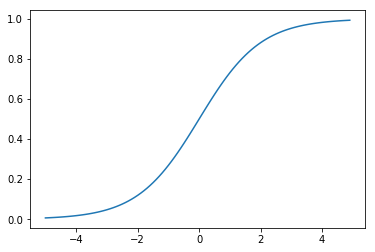
\includegraphics[scale=0.65]{sigmoidplot}
		\centering
	\end{figure}

	\textbf{Why is logistic function so important?}
	Because it can take any real input $x, (x \in R)$, whereas the output always takes values between 0 and 1, and hence is interpretable as probability.
	

	
\end{document}